\section{Exploration and Discussion}
\label{sec:discussion}
\subsection{Ablation Studies}
We further empirically explore various properties of \methodname{}. We conduct experiments  on the ADE20K dataset~\citep{zhou2019semantic}, which is a standard semantic segmentation dataset that includes a diversity of images and provides pixelwise segmentation of 150 different categories. 
We set the base learning rate to 0.004 and train the model for 240 iterations. We use SGD with momentum 0.9 and a polynomial learning rate scheduler with decay rate 0.9. We use \methodname{} with DPT and a smaller ViT-B/32 backbone together with the CLIP ViT-B/32 text encoder unless stated otherwise.


\textbf{Spatial regularization blocks.}
We first conduct an ablation study on the two variants of the spatial regularization blocks for cleaning up the output. 
We ablate the different types of blocks as well as stacking various numbers of blocks ($N \in [0, 1, 2, 4]$). The results are shown in Table~\ref{tab:ablation_arch}. We notice that a consistent improvement can be achieved by adding a few regularization blocks. The strongest improvement is achieved by stacking two \bottleneckblock{s}, an addition to the architecture that incurs little overhead.



\begin{table}[b!]
    \centering
    \scalebox{0.90}{
\begin{tabular}{c|c|cccc}
\toprule 
&&\multicolumn{4}{c}{\# depth}  \\
Block Type&Metric&0&1&2&4 \\
\midrule\midrule
&pixAcc [\%]&79.70&79.72&\textbf{79.78}&7.67\\
\depthwiseblock{}&mIoU [\%]&37.83&39.19&\textbf{39.45}&0.18\\
&pixAcc [\%]&79.70&79.64&\textbf{79.70}&79.68\\
\bottleneckblock{}&mIoU [\%]&37.83&39.16&\textbf{39.79}&38.78\\
\bottomrule
\end{tabular}
}
\caption{Ablation study on the depth of \bottleneckblock{} and \depthwiseblock{} before the last layer. For both Pixel Accuracy (pixAcc) and mIoU, higher is better. For depth=1, we directly feed the output to reshape without activation.}

    \label{tab:ablation_arch}
    % \vspace{-0.1in}
\end{table}

\begin{table}[b!]
    \centering
    \scalebox{0.90}{
\begin{tabular}{c|c|c|c|c|c}
\toprule 
Method&Backbone& Text Encoder (fixed) &embedding dimension &pixAcc [\%]&mIoU [\%] \\
\midrule\midrule
\methodname{}&ViT-B/32&ViT-B/32&512&79.70&37.83 \\
\methodname{}&ViT-B/32&ViT-B/16&512&79.77&38.69 \\
\methodname{}&ViT-B/32&RN$50\times4$&640&79.85&38.93 \\
\methodname{}&ViT-B/32&RN$50\times16$&768&\textbf{80.26}&\textbf{40.36} \\
\bottomrule
\end{tabular}
}
\caption{Ablation study on \methodname{} with fixed text encoders of different CLIP pretrained models. }



    \label{tab:ablation_textenc}
    % \vspace{-0.1in}
\end{table}

\textbf{Text encoders.} 
\methodname{} supports arbitrary text encoders in principle. We show the influence of using different text encoders in Table~\ref{tab:ablation_textenc}, where we ablate various encoders that are provided by the CLIP zero-shot image classification model~\citep{radford2021learning}. Note that all text encoders feature the same transformer-based architecture that purely operates on text. The main difference
between the encoders is the image encoder that was paired during CLIP pretraining (for example, the text encoder denoted by ``ViT-B/32'' was trained in conjunction with a ViT-B/32 image encoder) and the size of the embedding dimension.


We observe that using RN$50\times16$ achieves the best performance among all text encoders and surpasses the weakest ViT-B/32 text encoder by 2.5\%. We conjecture that this is because of the larger size of the embedding that is provided by this encoder.


\textbf{Comparison on a fixed label set.}
Language assistance helps boost the recognition performance on unannotated or unseen classes. However, there might be a concern that this flexibility hurts the performance on tasks that have a fixed label set. To test this, we train \methodname{} on ADE20K using the standard protocol on this dataset, where the training and test labels are fixed (that is, there are no unseen class labels at test time). We compare the results to highly competitive standard semantic segmentation models, including OCNet~\citep{yuan2020object}, ACNet~\citep{fu2019adaptive}, DeeplabV3~\citep{chen2017rethinking,zhang2020resnest}, and DPT~\citep{ranftl2021vision}. The results are listed in Table~\ref{tab:ablation_comp}. We find that \methodname{} performs competitively when using the RN$50\times16$ text encoder and incurs only a negligible loss in performance when compared to the closest fixed-label segmentation method (DPT).

\begin{table}[htb!]
    \centering
    \scalebox{0.90}{
\begin{tabular}{c|c|c|c|c}
\toprule 
Method& Backbone &Text Encoder&pixAcc [\%]&mIoU [\%] \\
\midrule\midrule
OCNet& ResNet101 &-&-& 45.45 \\
ACNet& ResNet101 &-&81.96& 45.90 \\
DeeplabV3& ResNeSt101 &-&82.07& 46.91 \\
DPT&ViT-L/16&-&\textbf{82.70}&\textbf{47.63} \\
\midrule
\methodname{}&ViT-L/16&ViT-B/32&82.46&46.28 \\
\methodname{}&ViT-L/16&RN$50\times16$&\textbf{82.78}&\textbf{47.25} \\
\bottomrule
\end{tabular}
}
\caption{Comparison of semantic segmentation results on the ADE20K validation
set. For \methodname{}, we conduct experiments with fixed text encoders of ViT-B/32 and RN$50\times16$ CLIP pretrained models.}



    \label{tab:ablation_comp}
\end{table}


\subsection{Qualitative Findings}
\label{sec:dis_qua}
We finally train \methodname{} on a mix of 7 different datasets~\citep{lambert2020mseg}, including ADE20K~\citep{zhou2019semantic}, BDD~\citep{yu2020bdd100k}, Cityscapes~\citep{Cordts2016Cityscapes}, COCO-Panoptic~\citep{lin2014microsoft,caesar2018coco},  IDD~\citep{varma2019idd}, Mapillary Vistas~\citep{neuhold2017mapillary}, and SUN RGBD~\citep{song2015sun}. Note that we train our model on the original label sets that are provided by these datasets  without any preprocessing or relabeling.
We follow the same training protocol as on ADE20K and train \methodname{} with a ViT-L/16 backbone and a ViT-B/32 text encoder 
for 200 epochs with a base learning rate of 0.004. If there are multiple labels for one class, we only use the first label that is provided during training. We select images from the web and show the results in Figure~\ref{fig:example_illustration23} to illustrate the use of the resulting model.



\begin{figure}
    \centering
     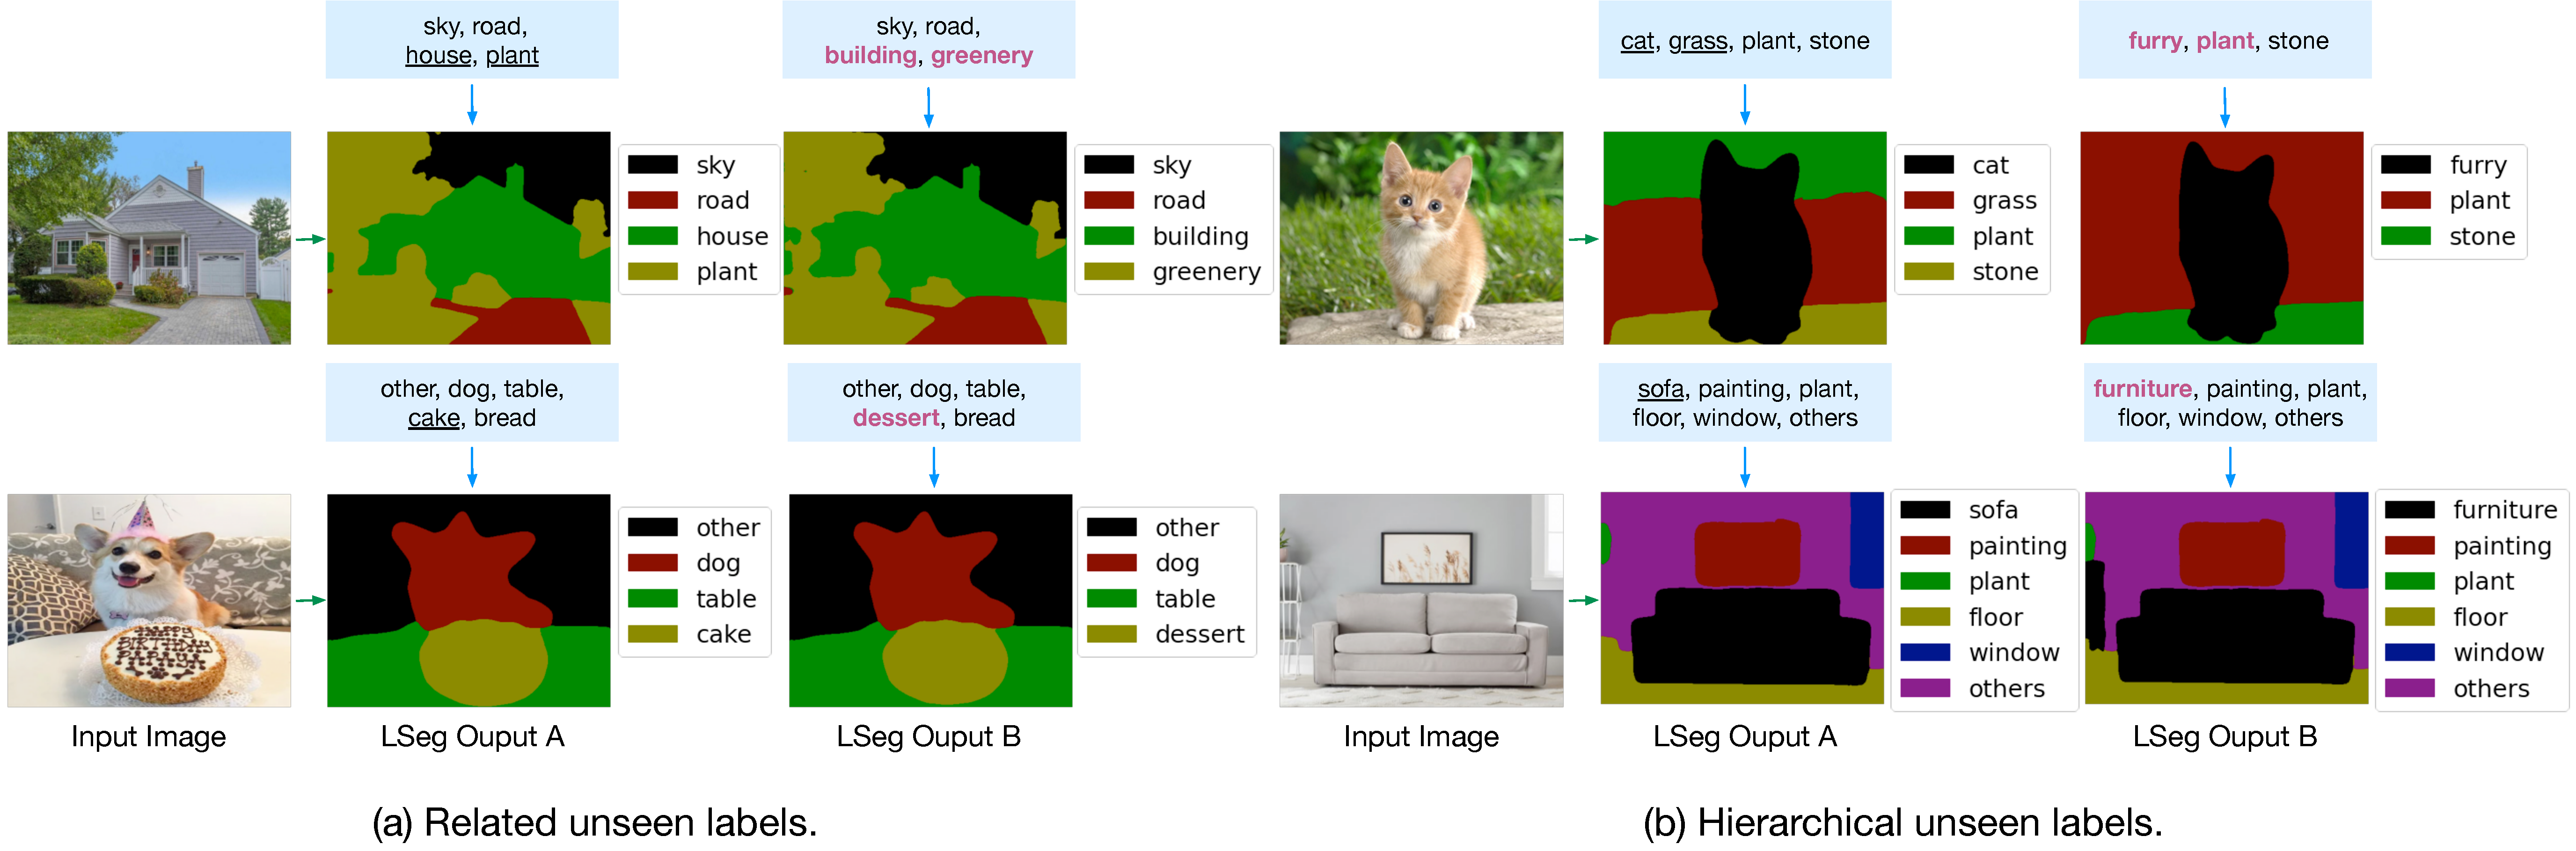
\includegraphics[width=\linewidth]{imgs/example_illustration23.pdf}
     \vspace{-0.2in}
     \caption{\methodname{} examples with related but previously unseen labels, and hierarchical labels. Going from left to right, labels that are removed between runs are \underline{underlined}, whereas labels that are added are marked in \textbf{\textcolor[HTML]{E45E9D}{bold red}}.}
     \label{fig:example_illustration23}
    \vspace{-0.2in}
\end{figure}


\textbf{Related but previously unseen labels.}
We illustrate some salient examples of the capabilities of \methodname{} to generalize to new classes in Figure~\ref{fig:example_illustration23}(a). In the first row, on the left we first start with the label set "sky", "road", "house", and "plant", and observe that the model is capable of segmenting the image into the provided classes. We then change the label "house" to "building" and the label "plant" to "greenery". The model produces a similar segmentation as before on this different but semantically related label set. This is despite the fact that the label "greenery" or even "green" was not present in any of the training images. A similar effect is shown in the second row, where \methodname{} successfully segments the image and correctly assigns the labels "cake" or "dessert" (again, the label "dessert" was not seen during training), while successfully suppressing the label "bread" which is both visually and semantically related.




\textbf{Hierarchical unseen labels.}
Figure~\ref{fig:example_illustration23}(b) demonstrates that \methodname{} can implicitly provide correct segmentation maps for hierarchies of labels. In the first row, the model is able to recognize the "cat", "plant" and "grass" segments of the image, as expected since these labels are present in the training set. When replacing "cat" with the label "furry", we notice that the model is able to successfully recognize this parent category (that is, most cats are furry, but not all furry objects are cats). Similarly, when removing the label "grass", we notice that the original "grass" region is merged into "plant", again an indication of an implicit hierarchy that is afforded by the flexibility of the text embeddings. The second row illustrates a similar scenario, where \methodname{} recognizes the sofa and other objects. However, the small shelf on the left is segmented as the unknown category "other". When we change "sofa" to "furniture", \methodname{} successfully identifies both the sofa and the small shelf as "furniture". Note that "furniture" never appeared in the training label set. 



\begin{wrapfigure}{R}{0.5\linewidth}
\vspace{-0.2in}
    \centering
     \subfigure[] {
		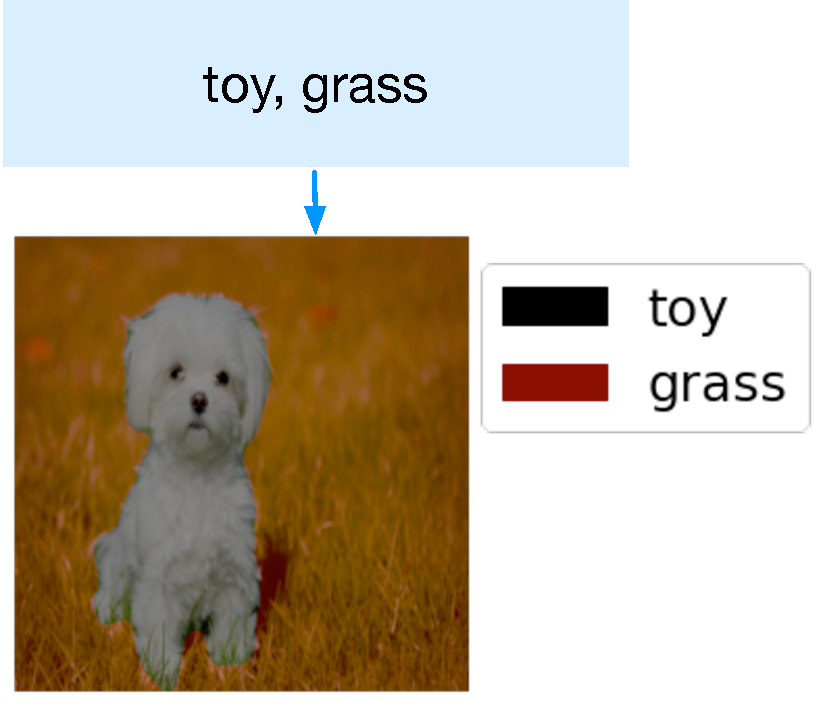
\includegraphics[width=1.2in, height=0.95in]{imgs/failurecases1.pdf}
		\label{fig:failurecases1}
	}
	\subfigure[] {
		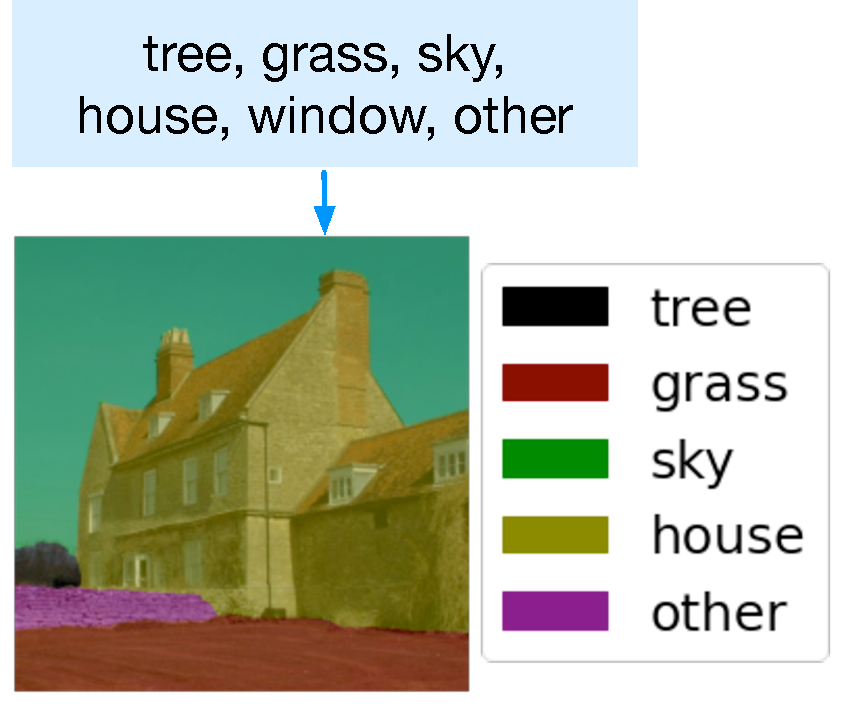
\includegraphics[width=1.2in, height=0.95in]{imgs/failurecases2.pdf}
		\label{fig:failurecases2}
	}
	\vspace{-0.15in}
    \caption{Failure cases. }
    \label{fig:failurecases}
    \vspace{-0.1in}
\end{wrapfigure}

\textbf{Failure cases.}
While \methodname{} in general achieves very promising results, we also observe some failure cases, as illustrated in Figure~\ref{fig:failurecases}. The left image illustrates that \methodname{} is only trained with positive samples from a class. When the test-time input labels do not contain any of the true labels for the corresponding pixel, the model assigns the highest probability to the closest label in the text embedding space. In this specific example, the model assigns the label "toy" since the visual features of the dog are apparently closer to "toy" than to "grass" in the embedding space and there is no other label that can explain the visual features.
A second failure case is shown on the right, where the model focuses on a single most likely object when multiple explanations are consistent with the label set. In this specific example, the windows of the house are labeled as "house" instead of window, even thought the label "window" is available as a choice.
We hope that these failure cases can inform future work, which could involve augmenting training with negative samples or building fine-grained language-driven semantic segmentation models that can potentially assign multiple labels when multiple explanations fit the data well.
